\chapter{Evaluation}
\label{chap:evaluation}
We implemented the algorithm explained in Chapter \ref{chap:testgeneration} as Eclipse plug--in and successfully tested it for a set of academic problems and performed a case study with a real world model from Airbus. We will point out that the transparent interchangeability of solvers is indeed one of the biggest advantages of the approach presented in this thesis. Also the limitations as well as missing but easily implementable features increasing the usability will be discussed in Section \ref{sec:evaluationLimitations}.
\section{Experiment Description}
\subsection{Runtime Measurement}
\label{sec:evaluationRuntimeMeasurement}
The total runtime of our algorithm is mainly influenced by two factors: The time necessary to solve one instance of the mathematical problem and the total count of problems to be solved during unit test generation. The total count of problems being solved depends on the model and the parameters used for the \nameref{sec:pathsearch}. For an acyclic activity diagram there is a finite number of control flow paths and abstract test cases. Assuming an activity diagram with a tree like control flow graph of depth 10 and a fanout of two in each node we get a total of $2^{10}$ abstract test cases. With normal breadth first or depth first path search we will have to solve one mathematical program for each abstract test case in order to obtain test data, or find out that it is an infeasible control flow path. In general we can say the number of control flow paths in an activity diagram grows exponentially with the number of decisions in the activity diagram; so does the number of problems being solved.\\
For the \nameref{sec:pathsearch} we examine the influence of three parameters on the overall runtime. That is the maximum path length, the maximum number of test cases, and the number of unchecked steps. All three of those parameters directly influence the amount of problems being solved in total and therefore influence the runtime. The maximum path length bounds the path search in depth and ensures the termination of the presented algorithm. The effect of this parameter had been explained in detail in Section \ref{sec:pathsearchDFS} For an activity diagram containing at least two different cycles the number of abstract test cases grows exponentially with the maximum path length. %Assume an activity diagram showing a loop, where in each iteration there is one decision with two possible control flows to take. Not after each node there are multiple outgoing edges, that means not every control flow in the control flow path has been choosen among several options, but the number of coises is linearly related to the maximum path length. Assume for the cyclic activity the cycle with the decision in it has the length of three no matter wich path had been taken inside the loop
The total amount of control flow paths found in a graph consisting of two alternative cycles of length $a$ can be calculated with Equation (\ref{eqn:MaxPathLength}) where $l_{MAX}$ denotes the maximum path length.
\begin{equation}\sum_{n=1}^{\lfloor l_{MAX}/a\rfloor}{2^n}\label{eqn:MaxPathLength}
\end{equation}
We expect the number of abstract test cases that need to be checked whether valid test data can be obtained for them to grow linearly with the parameter maximum number of test cases. The count of mathematical problems to be solved is expectedly the maximum number of test cases divided by the chance that any abstract test case found is an infeasible path. Consequently the overall runtime should depend linearly on the maximum number of test cases.\\
The parameter unchecked steps plays a role, when the early infeasible path recognition is activated (Section \ref{sec:EarlyInfeasiblePathRecognition}). The early infeasible path elimination will cut off a huge amount of abstract test cases when a sub--path is found to be infeasible, but it will also slightly increase the count of problems to be solved in the worst case. We again consider the tree like control flow graph with a fanout of two and a depth of ten. We have to solve one mathematical program for each abstract test case to obtain the test data and during the path search we will solve a mathematical program for several sub--paths. Assuming all $2^{10}$ abstract test cases are feasible paths the number of problems to be solved is approximately given in Equation (\ref{eqn:infeasiblePathRecognitionWorstCase}). $l_{UNCHCK}$ is the number of unchecked steps.
\begin{equation}
2^{10}+\sum_{n=l_{UNCHCK}+1, \Delta n=l_{UNCHCK}+1}^{10}{2^n}
\label{eqn:infeasiblePathRecognitionWorstCase}
\end{equation}
When we determine already after the third decision one of the $2^3$ control flow sub--paths to be infeasible that will reduce the total number of mathematical programs being solved by $\frac{1}{8}$. The less unchecked steps we use the more mathematical problems will be solved in vain if all paths are feasible, but the earlier we get the chance to eliminate infeasible paths the larger is the fraction of the search space we can directly cut off when an infeasible path is recognised. The optimal value for the unchecked steps parameter is a trade--off between solving unnecessarily many mathematical problems and not being able to cut of large portions of infeasible abstract test cases early enough.
\\
The runtime of a single solver run for models that require decidable problems with a tractable algorithm to be solved is usually below $0.1$ seconds. Also for problems with intractable algorithms the runtime stays below one second. A slight advantage in terms of solving speed has a large impact on the overall runtime since that is the part that consumes more than 95\% of the overall runtime. For undecidable problems there is the problem, that the heuristic might run forever and we need a good time limit for that. When the solver time limit is set to low then we will interrupt the solver many times to early although it would have found feasible test data for the current path. This will in total result in less test cases than could have been produced. When the time limit is too large we can waste houres waiting for the solver and realizing, that it will not return.\\
We measured the overall runtime of our algorithm transforming a UML \UMLType{Activity} into a compileable unit test for each of the models presented in the following section. For every example model and the case study we varied some of the parameters such as maximum path length, the maximum number of test cases, the number of unchecked steps, the used solver and its options. We plotted the graphs and discussed the experimental results.
\subsection{Mutation Testing}
For a selection of the Academic test models presented in Section \ref{sec:evaluationAcademicModels} we manually performed mutation tests. Therefore we selected a set of expressions from the implementation and defined mutation operators and applied them systematically to the selected expressions. For each manually generated mutant we ran the automatically generated test--suite and counted the failed tests.\\
A selected expression could be the predicate of a control flow statement or an assignment. As mutation operators we used the replacement of a single operation within the set of selected expressions. For example we replaced != by == or >= by <=. In every resulting mutant exactly one operation had been replaced. Since we produced one test--case for every possible control flow path in the activity diagram we expect the generated test to find most errors.
\section{Academic Examples}
\label{sec:evaluationAcademicModels}
In order to demonstrate the strength of our approach we built a set of test models. Each test model requires an instance of another mathematical programming problems presented in the \nameref{sec:Maths} to be solved in order to generate test data. For each test model we generated test cases with the depth first search explained in Section \ref{sec:pathsearchDFS} using the early infeasible path elimination explained in Section \ref{sec:EarlyInfeasiblePathRecognition}. We explain which problem the mathematical program generated for each test model is an instance of and justify which solvers are suitable to solve it. With each selected solver we generated test cases for the test model using different parameters for the depth first search and early infeasible path recognition. We measured the total runtime of our algorithm and plotted the runtime for different parameters graphically.\\
We also build a C-implementation for each academic test model and compiled and ran the generated unit tests against them and manually introduced some errors and checked whether they are detected by the generated test suite.\\
We will start with models, which require easy problems to be solved in order to obtain test data. By easy we mean decidable problems with a tractable algorithm. Then we will explain how we generated test data for problems, which require NP-hard problems to be solved. Finally we will also present models, which require an instance of an undecidable problem to be solved in order to obtain test data. That means we can only generate test data for them with heuristic methods.\\
Each solver is suitable for a set of problem classes, and for several problem classes there are multiple solvers that could be used. We performed some comparisons of different solvers in terms of runtime and the test data produced. For each presented test model we produced test data for all paths up to some maximum length.
For some models we show how much more effort in terms of runtime it is to generate boundary values as test data.\\
Finally we built a C implementation of the function modelled by the input to our algorithm and execute the generated test suite against this implementation. We also manually introduced some errors into the implementation and verified, that the produced test suite contains test cases that fail on those errors and that all test pass when the implementation is correct.
\subsection{Triangle Classificator}
\begin{figure}
\includegraphics[width=\textwidth]{./pics/TriangleLIN.pdf}
\caption{Triangle Classificator}
\label{fig:TriangleLin}
\end{figure}
\begin{figure}
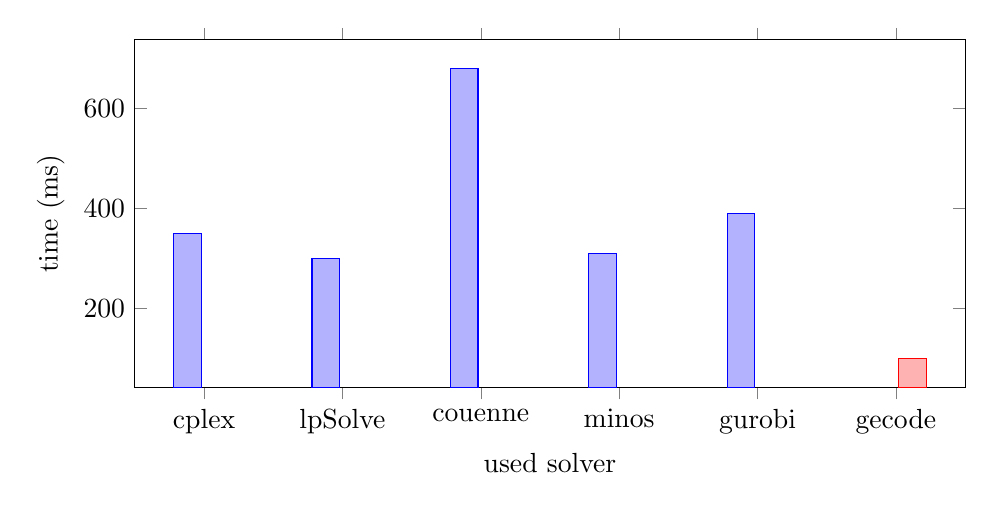
\begin{tikzpicture} 
\begin{axis}[ ybar,
width=\textwidth,
height=6cm,
ylabel={time (ms)},
xlabel={used solver},
xtick={0,1,2,3,4,5},
xticklabels={{cplex}, {lpSolve}, {couenne}, {minos}, {gurobi}, {gecode}},
]
\addplot coordinates {(0,350) (1,300) (2,680) (3,310) (4,390)}; 
\addplot coordinates {(5,100)}; 
\end{axis}
\end{tikzpicture}
\caption{Runtime of unit test generation using different solvers}
\label{fig:TriangleLinRuntime}
\end{figure}
We start with a model that contains only linear equalities and inequalities and variables in $\mathbb{R}$. Figure \ref{fig:TriangleLin} shows the activity diagram of a function taking three floating point values as input and returning a floating point value indicating whether the input variables could possibly be the side lengths of an equilateral, isosceles, or scalene triangle. The mathematical problem to solve for this model is a linear program and can be solved with the simplex method as implemented in cplex and lp\_solve or an interior point method as implemented by couenne, minos and gurobi. Generating test data for for every feasible abstract test case takes for every tested solver less than one second. There are in total 19 possible test cases resulting from this model. Figure \ref{fig:TriangleLinRuntime} shows the average runtime consumed for test generation from this model using the mentioned solvers.\\
We manually performed the mutation testing for this model. The following operator replacements have been made in the C-code: \verb=&&=$\rightarrow$\verb=||=, \verb=>=$\rightarrow$\verb�<=�, \verb=+=$\rightarrow$\verb=-=, \verb=||=$\rightarrow$\verb=&&=, \verb$==$$\rightarrow$\verb�!=�. This resulted in $20$ mutants of which 16 have been detected by our automatically generated test cases. That means 80\% of all mutants have been detected sucessfully.
\subsection{Triangle Classificator with Logical Constraints}
\begin{figure}
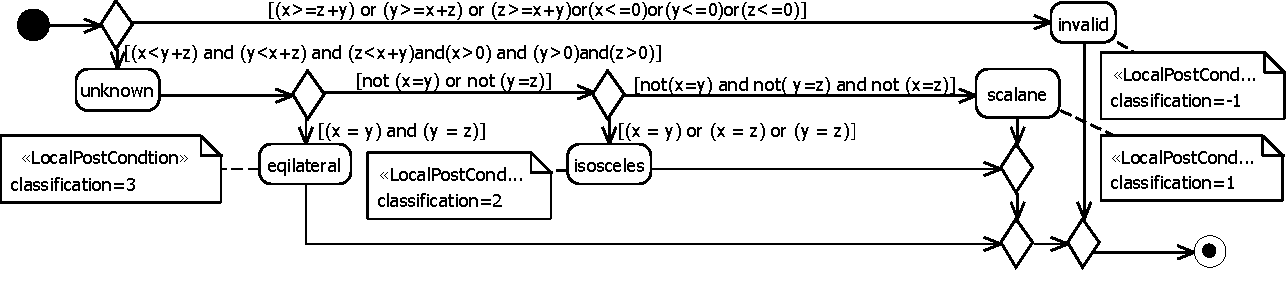
\includegraphics[width=\textwidth]{./pics/TriangleSMT.pdf}
\caption{Activity diagram of a triangle classificator using logical operations}
\label{fig:TriangleSMT}
\end{figure}
Since the formulation of the constraints by means of non-strict inequalities only is cumbersome we reformulated the model and used logical operations as well as strict inequalities in the guards and local post--conditions and yield the much more intuitive model depicted in Figure \ref{fig:TriangleSMT}. The variables are now all in the domain of integers and we used logical operations, thus this model will be transformed into an instance of an satisfiable modulo theories problem. Suitable solvers to solve instances of SMT are geode, ilogcp and jacop. In total there are 4 possible test cases to be found and our algorithm took 110ms to generate all of them using gecode. This time also shows up in the Figure \ref{fig:TriangleLinRuntime}.
\subsection{Binary Counter}
\begin{figure}
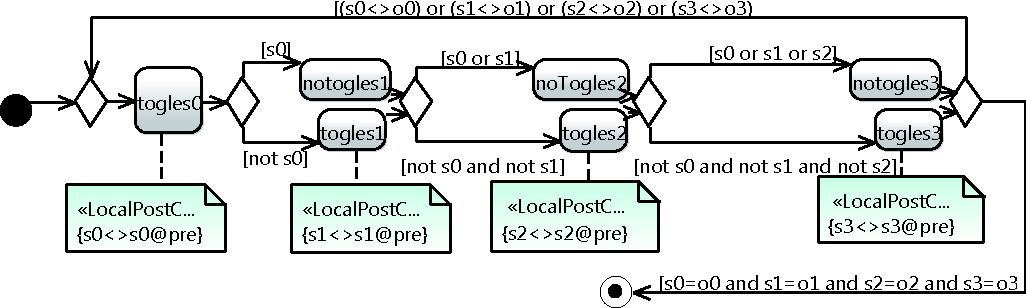
\includegraphics[width=\textwidth]{./pics/BinaryCounter.pdf}
\caption{Activity diagram of a binary counter incrementing a 4 bit register}
\label{fig:BinaryCounter}
\end{figure}
In Figure \ref{fig:BinaryCounter} we depict the activity diagram of a binary counter. The variables $s0$ to $s3$ hold the current state of the counter. The activity models a function with four input arguments $o0$ to $o3$ denoting the target counter state. During execution the the function will increment the binary counter stepwise until the current state of the counter is the same as the target counter state. Then the function returns. In contrast to the models presented so far this activity diagram is contains a cycle and consequently there are infinitely many abstract test cases and we need to bound the search.\\
All used variables are in $\mathbb{B}$ and we use logical operations in the formulation of constraints. In addition to the basic logical operations we also used the equality and inequality relation for boolean variables. The equality of two boolean variables x and y can be expressed as $x \land y \lor \neg x \land \neg y$ and the inequality as $\neg x \land y \lor x \land \neg y$. We consider the problem to solve in order to find test data for this activity an instance of the Boolean Satisfiability Problem (SAT) although the contained equalities and inequalities could be considered as expressions in a theory defining equality and inequality over boolean variables and thus the formulation could also be seen as SMT instance.\\
\subsubsection{Experiments}
\begin{figure}
\begin{tikzpicture}
\begin{axis}[
width=0.498\textwidth,
legend style={legend columns=2,at={(0.5,1.02)},
anchor=south},
xtick={10,20,30,40,50,60,70,80,90},
ytick={1e9,1e10,1e11,1e12,1e13},
yticklabels={1s,10s,100s,1000s,10000s},
ymajorgrids=true,
yminorgrids=true,
xmajorgrids=true,
xminorgrids=true,
xlabel={max path length},
ylabel={time},
xmin=5,
xmax=95,
%no markers,
ymode=log,
]
\addplot[densely dotted,no markers] table[x=PATHSEARCH_MAX_PATHLENGTH,y=time(ns)]{Experiment-DATA/BinaryCounterJacopSAT.csv};
\addlegendentry{JaCoP SAT};
\label{leg:jacopSAT};
\addplot[loosely dashed,no markers] table[x=PATHSEARCH_MAX_PATHLENGTH,y=time(ns)]{Experiment-DATA/BinaryCounterGecodeSAT.csv};
\addlegendentry{gecode SAT};
\label{leg:gecodeSAT};
\addplot[densely dashed,no markers] table[x=PATHSEARCH_MAX_PATHLENGTH,y=time(ns)]{Experiment-DATA/BinaryCounterGecodeSMT.csv};
\addlegendentry{gecode SMT};
\label{leg:gecodeSMT};
\addplot[solid,mark=x] table[x=PATHSEARCH_MAX_PATHLENGTH,y=time(ns)]{Experiment-DATA/BinaryCounterGecode+presolveSMT.csv};
\addlegendentry{gecode+presolve};
\label{leg:gecode+Presolve};
\addplot[solid,mark=+] table[x=PATHSEARCH_MAX_PATHLENGTH,y=time(ns)]{Experiment-DATA/BinaryCounterJacop+presolveSMT.csv};
\addlegendentry{jacop+presolve};
\label{leg:jacop+Presolve};
\end{axis}
\end{tikzpicture}%
\hspace{0.04\textwidth}
\begin{tikzpicture}
\begin{axis}[
width=0.498\textwidth,
nodes near coords,
xmin=5,
xmax=95,
xtick={10,20,30,40,50,60,70,80,90},
%y label style={at={1,0.5},anchor=west},
xlabel={max path length},
ylabel={total number of test cases},
%axis y line*=left,
]
\addplot+[mark=x,only marks,color=blue] table[x=PATHSEARCH_MAX_PATHLENGTH,y=PathsFound]{Experiment-DATA/BinaryCounterGecode+presolveSMT.csv};
\end{axis}
% \begin{axis}[
% width=0.498\textwidth,
% %nodes near coords,
% xmin=5,
% xmax=95,
% xtick={10,20,30,40,50,60,70,80.90},
% axis y line*=right,
% axis x line=none,
% ylabel near ticks,
% ylabel={total number of problems solved},
% ymode=log,
% ]
% \addplot+[mark=x,only marks,color=black] table[x=PATHSEARCH_MAX_PATHLENGTH,y=PATHSEARCH_TOTAL_SOLVER_RUNS,nodes=PathsFound]{Experiment-DATA/BinaryCounterGecode+presolveSMT.csv};
% \end{axis}
\end{tikzpicture}
\caption{comparison of runtime to generate one test case per feasible control flow path}
\label{fig:BinaryCounterRuntime}
\end{figure}
We performed several experiments with this example. First we transformed the the UML Activity into an activity test case graph and then into an AMPL model. We verified by hand, that the constraints in the AMPL model indeed expresses the same semantic as the OCL guard conditions and OCL local post--conditions in the UML model, and that every embedded OCL constraint contained in the input model shows up in the AMPL model. We implemented the C function, that is modelled by this activity diagram in order to run the generated unit tests against it later. Then we generated test cases for the model using two different solvers. Currently there are three solvers available for AMPL that can handle logical constraints: ilogcp, gecode, and jacop. Since for ilogcp a license is needed we performed our experiments with gecode and jacop. We used the depth first search algorithm with early infeasible path recognition as explained in Section \ref{sec:pathsearchDFS} to find test cases for this activity diagram. We generated all test--cases up to a control flow path length of 80. In the right graph in Figure \ref{fig:BinaryCounterRuntime} we see the total number of test cases found depending on the maximum path length.% and the amount of SAT instances that had to be solved to find those test cases
We also measured the overall runtime of the unit--test generation process. On the left hand side of Figure \ref{fig:BinaryCounterRuntime} we see the total runtime needed by our algorithm to find all test cases up to a given maximum path length using different configurations as explained in the following paragraphs. \ref{leg:gecode+Presolve} and \ref{leg:jacop+Presolve} show the runtime of of our algorithm using gecode and jacop for the model depicted in Figure \ref{fig:BinaryCounter}.
\paragraph{Effect of AMPL's Pre--Solve Phase}
AMPL tries to tighten the bounds of variables, eliminate some variables, and also eliminate some constraints not having any effect on the feasible set before passing the problem to the solver. This feature is called pre-solve phase and is activated by default. When causing trouble this pre--solve phase can be deactivated.% For the binary counter example we had to deactivate the presolve phase in order to generate test data for paths beyond a length of 60 since it caused AMPL to consume huge amounts of memory; and AMPL crashed when trying to allocate more than 2Gb. 
By deactivating the pre--solve phase the runtime of our algorithm increases by a factor of at least $100$. This is due to the fact, that most problem instances can already be identified as infeasible by the pre--solve phase after a few microseconds while solving the problem by a solver at least takes the time to start the solver in an external process. %We fixed this problem by just spawning a new AMPL process after it had crashed. 
In Figure \ref{fig:BinaryCounterRuntime} the \ref{leg:gecode+Presolve} plot denotes the runtime of the algorithm using gecode as solver with the pre--solve phase enabled and \ref{leg:gecodeSMT} plots the runtime with AMPL's pre--solve phase disabled. As we can see our algorithm is much faster with AMPL's pre--solve phase enabled.
\paragraph{Alternative Formulation of Constraints}
As we see the embedded OCL constraints contain equalities and inequalities over boolean variables in addition to the basic boolean operations. We replaced the equalities and inequalities with the equivalent boolean formula. Not all embedded OCL constraints were given in conjunctive normal form. Moreover the produced AMPL model will nevertheless still contain equalities, due to the continuity constraints that will be added automatically as explained in Section \ref{sec:addingContinuityConstraints}.% We considered it a too high manual effort to turn every OCL constraint into a perfect conjunctive normal form and explicitly stating all continuity constraints in conjunctive normal form within the UML model. Nevertheless 
We performed the runtime test also for the slightly modified model. Unfortunately we had to disable the pre--solve phase for this. The result is shown in the left graph in Figure \ref{fig:BinaryCounterRuntime}. \ref{leg:gecodeSAT} and \ref{leg:jacopSAT} indicate the runtime of our algorithm using gecode and jacop as solvers for the activity diagram modified as explained above. \ref{leg:gecodeSMT} depicts the runtime of our algorithm for the activity diagram as depicted in Figure \ref{fig:BinaryCounter} using gecode as solver and with AMPL's pre--solve phase disabled as well. When comparing \ref{leg:gecodeSAT} and \ref{leg:gecodeSMT} we see that for the solver it does not matter how the logical constraints are formulated. Those two plots are almost identical. % The divergence for maximum path lengths is not reproducable and is due to some random effects like java vm running its garbage collector.
\paragraph{Mutation Testing}
Also for this model we performed a manual mutation testing with the resulting test suite. We generated the test suite for all paths up to a maximum length of 40 using gecode as solver. The test suite contains 25 test cases. The C implementation of the binary counter is straight forward consisting of a do while loop and the bit flipping is done in the loop body. We applied the following mutations to the predicate of the do while loop in our source code: \verb=||=$\rightarrow$\verb=&&=, \verb$!=$$\rightarrow$\verb�==�, \verb$!=$$\rightarrow$\verb�<�, \verb$!=$$\rightarrow$\verb�>�. This results in 15 different mutants out of which 10 have been detected by the generated test suite. $66.\bar{6}\%$ of the generated mutants have been detected.
\paragraph{Discussion}
As already explained in Section \ref{sec:MathBooleanSat} the SAT is decidable but there is no tractable algorithm for it. Anyway our problem size will stay below the threshold where the solver needs more than a second to solve it. %Less than a second does not sound much, but to generate all test data for all control flow paths up to a given length many similar problems need to be solved. 
The number of solver invocations grows exponentially with the maximum path length when generating one test case per feasible control flow path through the activity diagram. In order to find the 49 possible test cases with a control flow path length of up to 70 our implementation solved 421901 SAT instances. Thus any slight advantage of one solver over the other or the way to formulate a constraint in terms of solving speed has an enormous impact on the overall runtime of the algorithm. As we saw during the experiment replacing equalities and inequalities with boolean formulas has no impact on the runtime but disabling AMPL's pre--solve phase had a negative influence on the overall runtime of our algorithm. Further more we can see a super exponential growth of the runtime of our implementation although we actually expected only exponential growth of runtime for our algorithm.
% \subsubsection{Non linear convex}
% solvable with every Solver implementing some version of Newton Algorithm on Sparse Matrices like Minos, Knitro or Quadratic programming approaches like in CPLEX.
\subsection{Exploding Tyres}
\label{sec:exampleModelNonConvex}
\begin{figure}
\label{fig:pumpTyre}
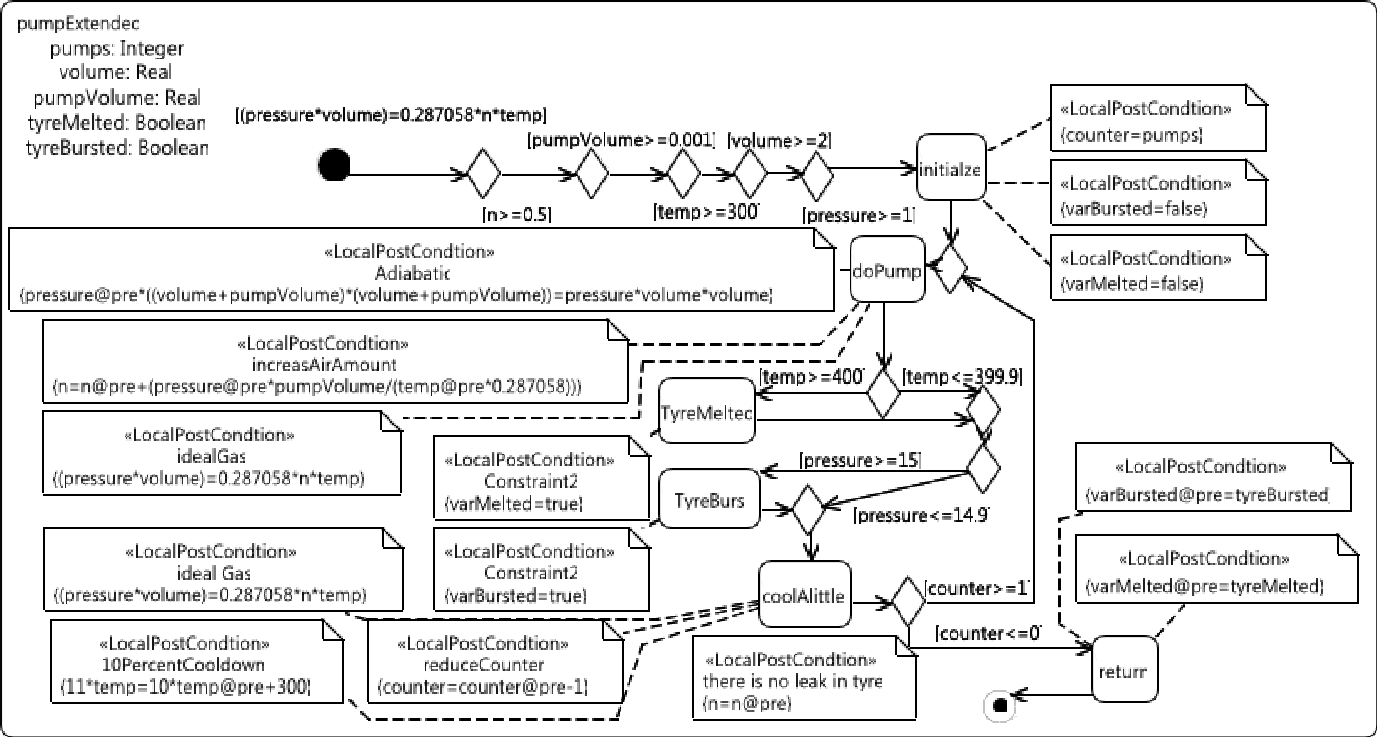
\includegraphics[width=\textwidth]{./pics/pumpTyre.pdf}
\caption{Activity Diagram with non convex mixed integer constraints}
\end{figure}
Figure \ref{fig:pumpTyre} shows an activity modelling the physical process of pumping air into a tyre. The relations between volume, amount of air ($n$), pressure, and temperature are described by the ideal gas equation. The equations for adiabatic compression of air during one pump stroke states a non-convex relation between these physical measures. Additionally we introduced the boolean variables tyreExploded and tyreMelted, which will be set when the pressure or temperature inside the tyre raised above a certain threshold. Moreover we introduce an integer loop counter that determines how many pump strokes will be executed. This model requires non--convex mixed integer problems to be solved in order to generate test data. The solver couenne from the COIN-OR project is suitable for this task. Couenne is the only solver we tested for non convex mixed integer constraint formulations.
\subsubsection{Runtime Measurement}
\begin{figure}
\begin{tikzpicture}
\begin{axis}[
width=0.498\textwidth,
legend style={legend columns=2,at={(0.02,0.98)},
anchor=north west},
%xtick={10,20,30,40,50,60,70,80,90},
ytick={1e8,1e10,1e12,1e14},
yticklabels={0.1s,10s,{1,000s},{100,000s}},
ymajorgrids=true,
yminorgrids=true,
xmajorgrids=true,
xminorgrids=true,
xlabel={max path length},
ylabel={time},
xmin=5,
xmax=75,
%no markers,
ymode=log,
]
\addplot[solid,no markers] table[x=PATHSEARCH_MAX_PATHLENGTH,y=time(ns)]{Experiment-DATA/ExplodingTyres_5sec.csv};
\addlegendentry{5sec};
\addplot[loosely dotted,no markers] table[x=PATHSEARCH_MAX_PATHLENGTH,y=time(ns)]{Experiment-DATA/ExplodingTyres_10s.csv};
\addlegendentry{10sec};
\addplot[densely dotted,no markers] table[x=PATHSEARCH_MAX_PATHLENGTH,y=time(ns)]{Experiment-DATA/ExplodingTyres_20sec.csv};
\addlegendentry{20sec};
\addplot[loosely dashed,no markers] table[x=PATHSEARCH_MAX_PATHLENGTH,y=time(ns)]{Experiment-DATA/ExplodingTyres_60sec.csv};
\addlegendentry{60sec};
\addplot[densely dashed,no markers] table[x=PATHSEARCH_MAX_PATHLENGTH,y=time(ns)]{Experiment-DATA/ExplodingTyres_10min.csv};
\addlegendentry{10min};
\addplot[solid,no markers] table[x=PATHSEARCH_MAX_PATHLENGTH,y=time(ns)]{Experiment-DATA/ExplodingTyres_2h.csv};
\addlegendentry{2h};
\end{axis}
\end{tikzpicture}
\begin{tikzpicture}
\begin{axis}[
width=0.498\textwidth,
legend style={legend columns=2,at={(0.02,0.98)},
anchor=north west},
%xtick={10,20,30,40,50,60,70,80,90},
%ytick={1e8,1e10,1e12,1e14},
%yticklabels={0.1s,10s,{1,000s},{100,000s}},
ymajorgrids=true,
yminorgrids=true,
xmajorgrids=true,
xminorgrids=true,
xlabel={max path length},
ylabel={number of test cases generated},
xmin=35,
xmax=75,
%no markers,
%ymode=log,
]
\addplot[solid,no markers] table[x=PATHSEARCH_MAX_PATHLENGTH,y=PathsFound]{Experiment-DATA/ExplodingTyres_5sec.csv};
\addlegendentry{5sec};
\addplot[loosely dotted,no markers] table[x=PATHSEARCH_MAX_PATHLENGTH,y=PathsFound]{Experiment-DATA/ExplodingTyres_10s.csv};
\addlegendentry{10sec};
\addplot[densely dotted,no markers] table[x=PATHSEARCH_MAX_PATHLENGTH,y=PathsFound]{Experiment-DATA/ExplodingTyres_20sec.csv};
\addlegendentry{20sec};
\addplot[loosely dashed,no markers] table[x=PATHSEARCH_MAX_PATHLENGTH,y=PathsFound]{Experiment-DATA/ExplodingTyres_60sec.csv};
\addlegendentry{60sec};
\addplot[densely dashed,no markers] table[x=PATHSEARCH_MAX_PATHLENGTH,y=PathsFound]{Experiment-DATA/ExplodingTyres_10min.csv};
\addlegendentry{10min};
\end{axis}
\end{tikzpicture}
\caption{measured runtime and number of generated test cases for different solver time limits}
\label{fig:ExplodingTyresRuntime}
\end{figure}
Non--convex mixed integer programs are in general undecidable consequently it may happen that a solver trying to solve an instance of an MIP runs infinitely long. It usually uses less than one minute to generate a feasible solution for one problem instance. But it also might run for a very long time or even infinitely long. 
%Repetition from section Experiment Description
%Consequently we need to set a suitable time limit after which the solver shall terminate and we assume the currently examined control flow path as infeasible. When the time limit is chosen very small the test generation is faster but on the other hand we will also consider several paths as infeasible although there would be a solution for the corresponding problem instance. When setting a larger time limit to we will certainly find a solution more often and thus generate more Test cases but the overall runtime will grow. 
In Figure \ref{fig:ExplodingTyresRuntime} we depict the overall runtime of the test generation for this model using couenne. For each plot we used the time limit for the solver printed in the legend. On the right hand side of Figure \ref{fig:ExplodingTyresRuntime} we depict the amount of test cases found depending on the time limit and the maximum path length. Up to a path length of 30 all problem instances had been solved or found infeasible after less than 20 seconds, thus the set time limits did not make a difference in the runtime as well as for the number of test cases found up to a maximum path length of 30. Comparing the run time of our algorithm with different time limits for the maximum path length of 60 we recognise, that increasing the time limit from 20 seconds to 60 seconds increased the overall runtime by a factor of 2.78 and generated 17 more test cases those are 9.2\% more test cases. Increasing the time limit from 60 seconds to 600 seconds increased the overall runtime by a factor of 7.67 and produced 11 additional test cases this is only 5.4\% more test cases. We see that increasing the lime limit for the solver masively increases the overall runtime, but we gain only very little more test cases for that. So we would recommend to use 10 to 20 seconds as time limit for couenne.
\subsubsection{Generating Boundary Values}
using the naive approach explodes solving time and two step boundary value generation using local search is good.
% \subsubsection{Constraint Programming}
% ILOGCP, Gecode or transformation possible
% \paragraph{Integer arithmetic only} Gecode
% \paragraph{linear mixed Integer arithmetic} IlogCP
% \begin{figure}
% \label{fig:classifyTriangle}
% 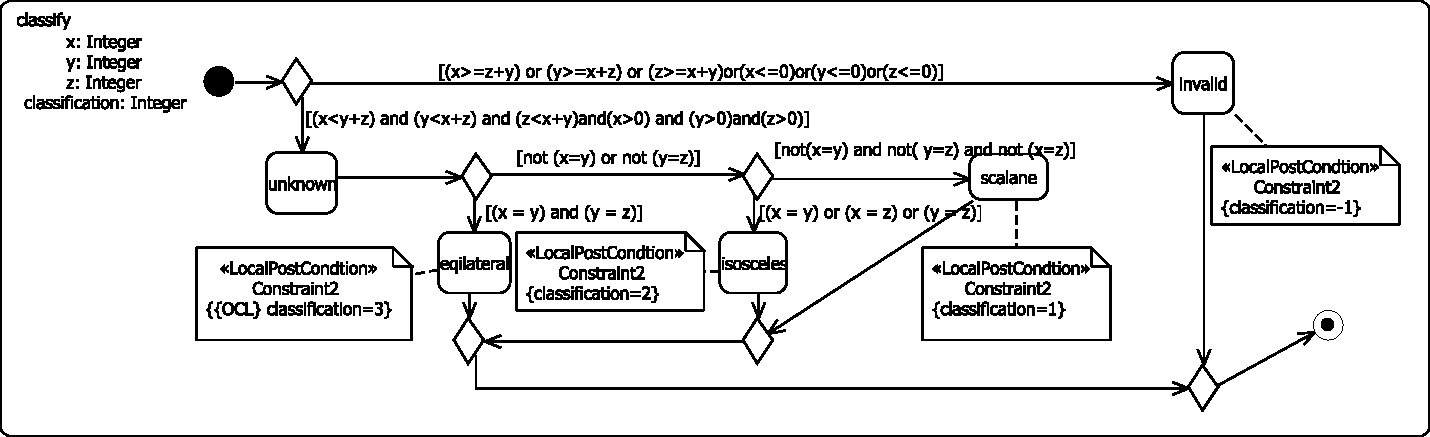
\includegraphics[width=\textwidth]{./pics/TriangleClassificator.pdf}
% \caption{Activity Diagram with non convex mixed integer constraints}
% \end{figure}
% \paragraph{nonlinear mixed Integer arithmetic}
% really really really problematic. Currently the only way is to transform the Activity Test Case Graph to remove the Logical Operations in favour of parallel or sequential Control Flows with guards. Use COUENNE.
\subsubsection{Running the Generated Test Cases}
We have implemented the modelled function in C and successfully ran the generated test cases against it. Although we did not do it systematically for this model we did a few mutation tests for the test cases generated from this model. The error propagation of very small errors in the floating point calculations is especially interesting. We see in the model there is a loop and in every round the values for temperature, pressure, amount of air (n) are updated depending on the values of those measures before. Consequently, when one of the calculations has a small error the error will be propagated to all three of those measures and we see a lot of failed tests due to just one wrong statement. Also for longer test cases taking the loop multiple times the introduced error is potentiated. In an experiment an error of 0.1 \% per loop iteration caused after 5 iterations an error of more than 0.5\%. Also reordering of statements introduced huge errors in all three measures. And finally eaven non optimal calculation plans did cause several test cases to fail, due to introduced rounding errors. One might think, that the new temperature after the coolAlitle action could be computed either as \verb$temp = (10 * temp + 300) / 11 ;$ or as \verb$temp = 10 * temp / 11 + 300 / 11 ;$. But the automatically generated test cases revealed that those two expressions do not produce the same results. The rounding errors of the second version causes all generated test cases to fail.
\section{Case Study PAX Model}
\label{sec:evaluationCaseStudy}
Additionally to the artificial test models demonstrating the use of our method for different kinds of constraints we also performed a case study with a real world model. We tested our implementation on a model modelling the PAX call system from Airbus. Out of the model of the complete product we selected an activity diagram modelling the interaction of the PAX call system with the \textbf{I}n \textbf{F}light \textbf{E}ntertainment (IFE) system. The selected \UMLType{Activity} contains 21 \UMLType{Actions}, 24 \UMLType{ControllNodes}, and two \UMLType{LoopNodes}. Furthermore there are eight \UMLType{DataStoreNodes} representing function local variables. The model was originally created with Artisan Studio, and used to generate a C-implementation from it with a proprietary code generator from Atego\textsuperscript{\textregistered}. The branching conditions and the code body of each \UMLType{Action} is given in C--syntax. All assignments and conditions consist of linear equations and inequalities only. All variables are in the integer or boolean domain. Consequently the constraint satisfaction problem to be solved for test data generation is an integer linear program. The solvers cplex and lpsolve are perfectly suitable for this kind of problem. Couenne can also be used for this task.\\
The described algorithm has several parameters, which mainly influence the \nameref{sec:pathsearch}. We use this case study to evaluate the influence of those parameters on the runtime of the Algorithm. The examined parameters are the maximum length of control flow paths , the maximum amount of test cases to be generated, and the unchecked steps before an early infeasible path check is performed during the path search.
\subsection{Manual Adaptation}
In order to generate C++ unit test code with our Eclipse plug-in from the described model several pre--processing steps need to be performed manually. Those manually to perform steps are the conversion of the Model from Atego\textsuperscript{\textregistered } Artisan Studio into Eclipse UML, adding all constraints in OCL syntax, the guards and the local post--conditions, flattening the \UMLType{LoopNodes}, and replacing the \UMLType{DataStoreNodes} by \UMLType{Properties}.\\
Atego\textsuperscript{\textregistered} does not store models natively in xmi format but has an option for exporting models in xmi format. The Eclipse Modelling Framework natively uses the xmi format to store models. Each modelling tool uses its own implementation of the UML meta model and there are slight differences in the implementations making the created models incompatible with each other. In order to import the model from Artisan in Eclipse we manually need to remove some objects not recognised by Eclipse and correct some typing errors in the xmi file. Then we can load the XMI and browse the model with the Eclipse Modelling Framework.\\
Every \UMLType{Action} is associated with a C-code snippet that is used for code generation. There are not yet \UMLType{Constraints} specifying the pre and post--conditions of each \UMLType{Action} in OCL. Also the \UMLReference{guards} do not contain OCL queries. We make an educated guess to add \UMLReference{guards} and \UMLReference{localPostconditions} reproducing the semantics of the C-code snippets contained in the original model. The original model used local C-struct variables modelled by the \UMLType{DataStoreNodes} contained by the \UMLType{Activity}. Our implementation can handle primitive data type variables modelled by \UMLType{Properties}, consequently we created one \UMLType{Property} per field of a struct variable. The original model also used arrays. We emulated the behaviour of an indexed collection by allowing all variables depending on an index to change to an arbitrary value whenever the index is changed. This may produce wrong behaviour but seemed fair enough to evaluate our algorithm. The \UMLType{DataStoreNodes} will be ignored by our algorithm.\\
The \UMLType{LoopNodes} contain further model elements in their \UMLReference{bodyPart} reference. Those elements from the \UMLReference{bodyPart} are directly included into the parent \UMLType{Activity} the \UMLType{InitialNode} and \UMLType{FinalNodes} of the loop body are replaced by decision nodes and directly connected to every element that was connected to the \UMLType{LoopNode}. In order to preserve the loop semantic a control flow from every final node of the body to the initial node of the body is added and decorated with a \UMLReference{guard}.\\
The function specifying which control flow to take after each \UMLType{Action} is \emph{well--defined} and \emph{defined} over the complete domain. Well--defined means there is no possible state in which more than one guard evaluates to true, and defined over the complete domain means that there is no value assignment for which all guards of the outgoing \UMLType{ControlFlows} evaluate to false.
\subsection{Runtime Experiments}
\begin{figure}
\begin{tikzpicture}
\begin{axis}[
width=0.49\textwidth,
legend style={at={(0.02,0.98)},anchor=north west},
ylabel={time},
xlabel={max path length},
ytick={10000000000,60000000000,600000000000,3600000000000},
yticklabels={10s,1m,10m,1h},
ymajorgrids=true,
yminorgrids=true,
xmajorgrids=true,
no markers,
ymode=log,
]
\addplot table[x=PATHSEARCH_MAX_PATHLENGTH,y=time(ns)]{Experiment-DATA/CaseStudyRuntimeCplex.csv};
\addlegendentry{Cplex};
\addplot table[x=PATHSEARCH_MAX_PATHLENGTH,y=time(ns)]{Experiment-DATA/CaseStudyRuntimeLPSolve.csv};
\addlegendentry{lpSolve};
\addplot table[x=PATHSEARCH_MAX_PATHLENGTH,y=time(ns)]{Experiment-DATA/CaseStudyRuntimeCouenne.csv};
\addlegendentry{couenne};
\end{axis}
\end{tikzpicture}%
\begin{tikzpicture}
\begin{axis}[
width=0.49\textwidth,
xlabel={unchecked steps},
xmax=15,
ylabel={time},
ytick={10000000000,60000000000,600000000000,3600000000000,864e11},
yticklabels={10s,1m,10m,1h,1d},
no markers,
legend style={legend columns=3,overlay,at={(0.5,1.02)},anchor=south},
ymajorgrids=true,
yminorgrids=true,
xmajorgrids=true,
xminorgrids=true,
no markers,
ymode=log,
] 
\addplot table[x=PATHSEARCH_UNCHECKED_STEPS,y=time(ns);]{Experiment-DATA/CaseStudyUncheckedSteps40.csv};
\addlegendentry{40};
\addplot table[x=PATHSEARCH_UNCHECKED_STEPS,y=time(ns);]{Experiment-DATA/CaseStudyUncheckedSteps50.csv};
\addlegendentry{50};
\addplot table[x=PATHSEARCH_UNCHECKED_STEPS,y=time(ns);]{Experiment-DATA/CaseStudyUncheckedSteps60.csv};
\addlegendentry{60};
\addplot table[x=PATHSEARCH_UNCHECKED_STEPS,y=time(ns);]{Experiment-DATA/CaseStudyUncheckedSteps70.csv};
\addlegendentry{70};
\addplot table[x=PATHSEARCH_UNCHECKED_STEPS,y=time(ns)]{Experiment-DATA/CaseStudyUncheckedSteps80.csv};
\addlegendentry{80};
\addplot table[x=PATHSEARCH_UNCHECKED_STEPS,y=time(ns)]{Experiment-DATA/CaseStudyUncheckedSteps90.csv};
\addlegendentry{90};
\end{axis}
\end{tikzpicture}%
%\end{center}
\caption{Runtime of Test Generation }
\label{fig:RuntimeExperiments}
\end{figure}
%The implemented algorithm has several properties influencing the exact execution of the \nameref{sec:pathsearch}. 
In this section we examine the influence of the used solver, the maximum path length, and the maximum number of test cases on the runtime of our algorithm using the case study model as input. The expected effects of those parameters on the overall runtime have already been discussed in Section \ref{sec:evaluationRuntimeMeasurement}.\\
In Figure \ref{fig:RuntimeExperiments} we plotted on the left hand side the the runtime needed depending on the maximum path length. We performed this experiment for different Solvers. For abstract test case generation the depth first search with early infeasible path elimination and 2 unchecked steps has been used. As we see lpsolve produced the fastest results directly followed by cplex. Using couenne our algorithm takes round about 3 times the runtime consumed using lpsolve. This might be because couenne is actually suitable for the much more general mathematical problem of non-convex mixed integer programs and thus is not perfectly specialized for linear mixed integer programs. The runtime grows almost perfectly exponential with the maximum path length. With a closer look at the graph we can see, that it is slightly super exponential. This might be caused by effects that are inherent to the computing architecture executing the implementation of our algorithm.\\
On the right hand side of Figure \ref{fig:RuntimeExperiments} we plotted the overall runtime of our algorithm depending on the unchecked steps parameter of the early infeasible path elimination. We used cplex as solver for this experiment and repeated the experiment for different maximum path lengths. As we can see from the plots, up to a maximum path length of 50 it is not beneficial using early infeasible path elimination when generating test cases for the case study model. With longer maximum path lengths the impact of a well configured early infeasible path elimination grows. For a maximum path length of 90 our algorithm configured with the optimal value for the unchecked steps parameter takes less than one hour to generate all test cases, while it takes several days when unchecked steps is set to 5 or 6. 
%It is perfectly plausible when we assume p to be the conditional probability that by appending one control flow to a feasible path the new path is also feasible. In every step we can select one of two control flows to be appended to the current path. Now when we check after $\Delta$ steps we will have in total $2^{\Delta}$ paths that need to be checked for feasibility and each of them will have a chance of $p^{\Delta}$ of being feasible. Consequently after another $\Delta$ control flows being appended to each feasible path there will be on average another $p^{\Delta}*2^{2\Delta}$ paths that need to be checked for feasibility. The total amount of mathematical programs solved performing an ifeasible path check every $\Delta$ steps and 
% \begin{tikzpicture} \begin{axis}[%ymode=log,
% ] 
% \addplot[yellow,domain=1:5] {((1-0.99^x)*2^(2*x)-2^x)/2^(x)};
% \addplot[black,domain=1:5] {((1-0.9^x)*2^(2*x)-2^x)/2^(x)};
% \addplot[green,domain=1:5] {((1-0.8^x)*2^(2*x)-2^x)/2^(x)};
% \addplot[blue,domain=1:5] {((1-0.7^x)*2^(2*x)-2^x)/2^(x)}; \addplot[red,domain=1:5] {((1-0.5^x)*2^(2*x)-2^x)/2^(x)}; 
% \end{axis} \end{tikzpicture}
% \begin{tikzpicture} \begin{axis}[%ymode=log,
% ] 
% \addplot[yellow,domain=1:5] {((1-x^1)*2^(2*1)-2^1)/2^(2*1)};
% \addplot[black,domain=1:5] {((1-x^2)*2^(2*2)-2^2)/2^(2*2)};
% \addplot[green,domain=1:5] {((1-x^3)*2^(2*3)-2^3)/2^(2*3)};
% \addplot[blue,domain=1:5] {((1-x^4)*2^(2*4)-2^4)/2^(2*4)}; \addplot[red,domain=1:5] {((1-x^5)*2^(2*5)-2^5)/2^(2*5)}; 
% \end{axis} \end{tikzpicture}
% As already explained in Section \ref{sec:pathsearch} and Section \ref{sec:EarlyInfeasiblePathRecognition} there are two parameters that ensure the termination of the \nameref{sec:pathsearch}. Those are the maximal path length and the maximum amount of test cases generated. It is quite obvious that the number of test cases found may depend exponentially on the maximal control flow path length. We assume, that the path search algorithm described in Section \ref{sec:pathsearchDFS} will find abstract test cases at a constant rate. According to this assumption the runtime of the algorithm should linearly depend on the amount of test cases generated. Thus the maximal number of test cases to be found should be correlated linearly to the overall runtime of the algorithm, and we expect the maximum control flow path length to be exponentially correlated to the runtime of the test generation algorithm. \\
%There is also one parameter steering the early infeasible path elimination. That is the amount of unchecked steps. Calling the solver is very expensive in terms of runtime. To check whether the current control flow path is infeasible we need to solve the corresponding constraint satisfaction problem. If we check every time one control flow has been added to a control flow path we will eliminate infeasible paths as soon as possible, but will also call the solver unnecessarily often to find out that one constraint added did not make the path infeasible. If we perform a check for infeasible control flow paths after every tenth decision passed we will have to check at least $2^{10}$ control flow paths whether they are feasible or not, where several of them could have been eliminated much earlier by computing much less constraint satisfaction problems. We pay special interest to the influence of the number of unchecked decisions before control flow paths are checked for feasibility. We assume, that there will be a minimum of runtime for some number of unchecked decisions.
%Complex data types we added one \UMLType{Property} per field in a variable.
%When the Model was correctly imported we need to add to each \UMLType{Action} those local post--conditions that describes the assignments done in the C-code associated with that \UMLType{Action}
%I could do a case study with the Airbus PAX call model from Atego\textsuperscript{\textregistered }.
\section{Verification of the Implementation}
We claim that the Eclipse plug--in built aside this thesis implements the algorithm explained in \nameref{chap:testgeneration}. This claim is validated manually by checking each step separately. We use the Academic Example models presented in Section \ref{sec:evaluationAcademicModels} as test cases to verify each transformation described in \nameref{chap:testgeneration}. From each input model we created manually the intermediate artefacts that should have been created according to the specification and compared them to the intermediate artefacts produced by the plug-in.
\section{Limitations}
\label{sec:evaluationLimitations}
Besides all the things we demonstrated that our algorithm is capable of there are also some things that we can not do. We divided this section into three parts first we will show up which features will provably be never realizable due to theoretical constraints. Those are the Theoretical limitations. Then we will name some features that could have easily been added to the presented method but are not described throughout this thesis. And finally we will show up which features could be added if the used libraries and external tools would provide better support.
\subsection{Theoretical Limitations}
The most important source of limitations is the undecidability. Although we were able to produce some valid test cases for a model using undecidable formulas in their local post--conditions and guards we will never be an algorithm that is able to automatically produce one test case for every possible abstract test case in the activity test case graph generated from such an activity diagram. There will always be some special cases where any applied heuristic will neither find a feasible solution nor it can generate a proof that there is no solution to the mathematical program to be solved in order to generate the test data.\\
If all constraints in the model are instances of a decidable problem it may still be the case, that the algorithm is intractable. In such a case we will have problems with the scalability of our approach when using exact solvers. The only way out would then be to use a solver implementing a tractable heuristic instead of an exact method to solve the mathematical program, which in turn might report some paths to be infeasible although there exists a solution that would have been found by the exact method.\\
Another limitation to scalability is the combinatorial explosion of possible control flow paths through an activity test case graph with growing path length. Unless one decides to use only a special subset of all possible control flow paths as abstract test cases the algorithm will always suffer from exponential runtime and it will also produce a number of test cases that grows exponentially with the maximum path length.
% able to produce one test case for every feasible pathall possible test cases for 
% undecidability of non--linear arithmetic over invite sets and Exponential runtime for Constraint solving algorithms for some formulations
\subsection{Limitations of the Implementation}
Several features of the UML could have easily been supported by our approach. We concentrated on the core idea in this thesis and created a good software architecture allowing later extensions of our initial concept.\\
Possibly missing features are support or hirarchical modelling with \UMLType{ActivityCallActions} or \UMLType{StructuredActivityNodes}. Further more the input language currently does not support operations on variables with a type other than boolean, integer or real. Support for arbitrary datatypes such as enums or objects can be added by modifying the \nameref{sec:atcg2Ampl} step of our algorithm.\\
Currently as constraints only the \UMLType{ControlFlows} \UMLReference{guard} conditions and the \UMLType{Actions} \UMLReference{localPostConditions} are considered. All possible ways to embed invariants and several other ways to embed pre and post conditions into an UML model are ignored. This could be fixed in the \nameref{sec:Normalisation} step of the presented algorithm.\\
Finally it might not be in the interest of the industrial user that for larger models the test case generation with our algorithm may take several days and produce several thousand test cases (for the case study we had produced 83,000 test cases in 13 hours). The generation of a moderate amount of test cases ensuring full code coverage of the implementation or fulfilling some coverage criterion on the input model might be more desirable. To achieve this a modification of the \nameref{sec:pathsearch} is necessary.
%no structured activity nodes, no invariants, not completely implemented test goal management.
\subsection{Limitations of used Tools}
AMPL's normal use case is mathematical optimisation and throughout the years several additional features have been added to the language. Unfortunately we do not know about any solver capable of handling all constraints that can be expressed with AMPL. Especially support for SMT formulations using non linear convex arithmetic as background theory is missing. With the commercial solver IlogCp it is possible to delegate the solution of sentences in a background theory to cplex which is capable of solving linear mixed integer programs and quadratic mixed integer problems which is another specialization of convex mixed integer programming.\\
The used Eclipse OCL parser by default supports a minimal set of arithmetic operations consequently it is not possible to support arbitrary arithmetic without modifying the Eclipse OCL parser.\\
In theory the xmi interchange format should enable the exchange of UML models between different modelling tools. Unfortunately the import of UML models into Eclipse exported by Artisan Studios does not yet work flawless. Thus our implementation is merely limited to be applied to models generated by Papyrus, unless one is willing to spend some manual work to make the exported UML model of third party tools compliant to Eclipse UML. 
% tool for buissness use
% XMI interchange format does not work always LOTS OF BUGS!!!!
% \section{Further Ideas}
% 
% The first thing we recommend to to 
% 
% We recommend to extend the described subset 
% There is no good reason for using OCL as the specification language in order to ease the constraint solving prolog could directly be used as language to specify constraints in a UML Model.


